\section{Vorgehensplan zur Zusicherung ethischer Werte}\label{sec:massnahmen}
Die Umsetzung der in \autoref{sec:def_ethischer_werte} definierten ethischen Werte soll entlang eines üblichen Softwarelebenszyklus \cite[S. 64]{broy2013} erfolgen, da die ethischen Probleme in allen Phasen Beachtung finden müssen.

\begin{figure}[ht]
    \centering
    \frame{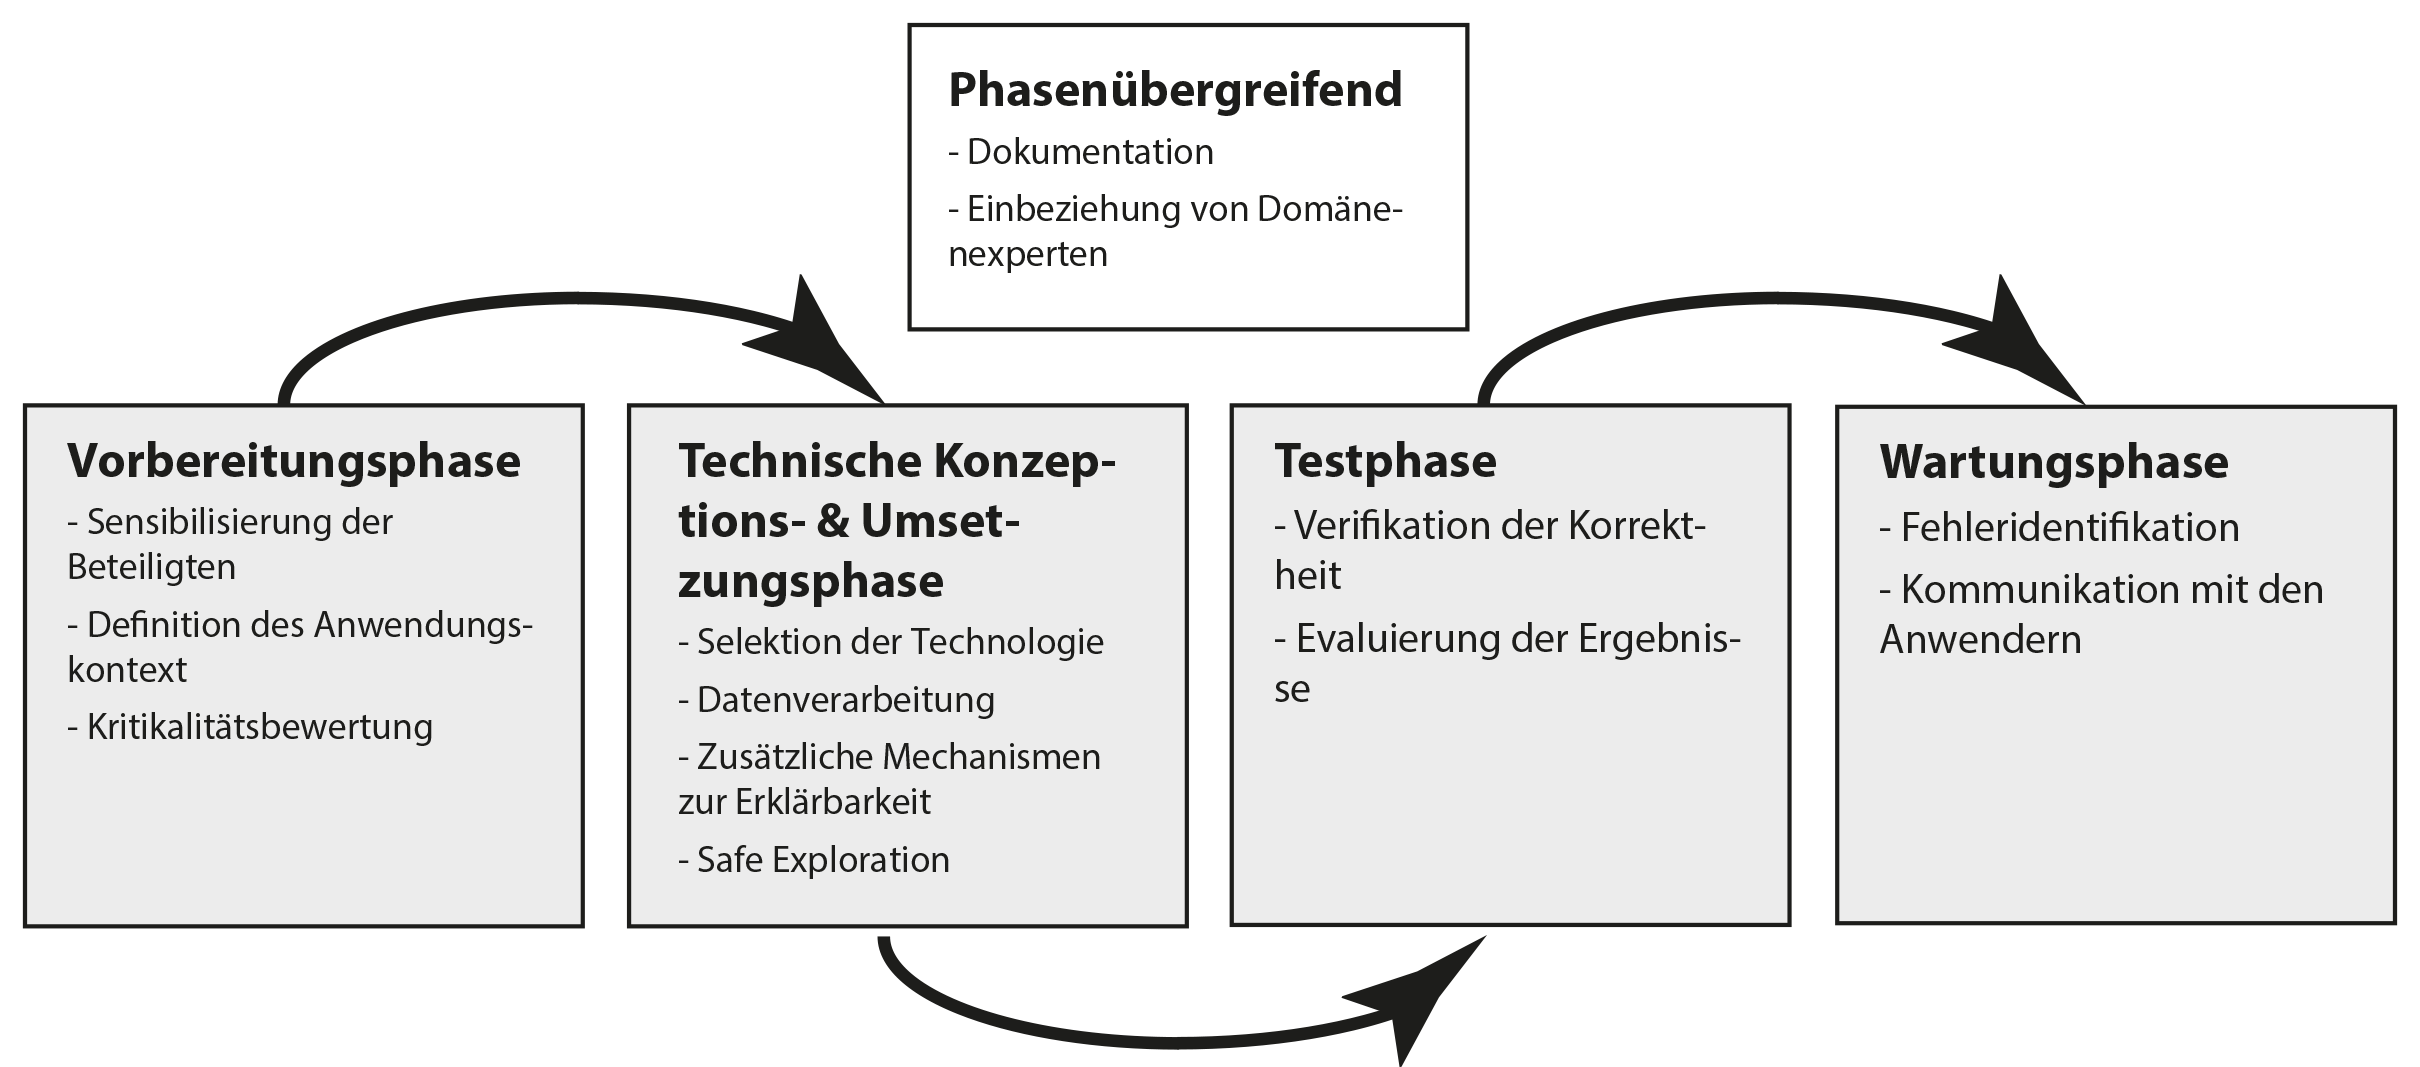
\includegraphics[width=\textwidth]{graphics/guidelines.png}}
    \caption{Phasen und jeweilige Maßnahmen der Zusicherung ethischer Werte.}
    \label{fig:guidelines}
\end{figure}

Die in \autoref{fig:guidelines} skizzierten Maßnahmen werden im Folgenden hinsichtlich der ethischen Werte begründet.
Das Vorgehen soll kompatibel mit den meisten Vorgehensmodellen sein, indem die Phasen so allgemein gefasst sind, dass sie nahezu in allen Vorgehensmodellen in irgendeiner Form vorkommen.
Die Phasen können parallel zu den jeweiligen Phasen im Vorgehensmodell durchgeführt werden.
Viele Maßnahmen behalten ihre Gültigkeit über die jeweilige Phase hinweg, sollten jedoch spätestens ab der vorkommenden Phase beachtet werden.
Es wird kein spezieller Fokus auf einzelne Domänen gesetzt.
Stattdessen werden allgemeine Hinweise und Möglichkeiten aufgelistet, wodurch eigene Maßnahmen abgeleitet werden können.
Viele der Maßnahmen beziehen sich im Speziellen auf sicherheitskritische Anwendungen.
Innerhalb der Phasen wird zunächst das Ziel der jeweiligen Phase erläutert und anschließend technische und organisatorische Maßnahmen vorgestellt.
Ziel dieses Vorgehens ist die Definition von Leitlinien, die mit den in \autoref{sec:def_ethischer_werte} vorgestellten Werten kompatibel sind und in bestehende Prozesse integriert werden können.
\ab 
Vorweg werden Maßnahmen eingeführt, die phasenübergreifend gültig sind und ggfs. innerhalb der einzelnen Phasen spezieller betrachtet werden.
So ist Dokumentation in jeder Phase ein wichtiges Mittel, um das Verhalten nachvollziehen zu können, Vertrauen durch Transparenz aufzubauen und Verantwortung zuordnen zu können.
Welche Informationen dabei in den einzelnen Phasen relevant sind, wird an passender Stelle jeweils beschrieben.
Alle dokumentierten Informationen sollten langfristig und in einem menschlich lesbaren Format gespeichert werden.
Optimalerweise wird die Dokumentation ähnlich wie eine Lizenzangabe mit der Software bzw. dem Agenten ausgeliefert.
In dem Fall muss die Dokumentation möglichst klar und dem Wissensniveau des Anwenders entsprechend formuliert sein.
Neben einer ausführlichen Dokumentation ist phasenübergreifend eine Miteinbeziehung von Domänenexperten sinnvoll \cite[S. 12 ff.]{gottesman2018}.
Domänenexperten können schon während des Entstehungsprozesses Einfluss auf die inhaltliche Korrektheit ausüben.
Um ethisches Handeln zuzusichern, kann zudem z.B. in allen Entwicklungsschritten eine explizite Aufforderung der Übereinstimmung der formulierten Werte und der moralischen Prinzipien der Mitarbeiter gefordert und die Zustimmung oder mögliche Mängel dokumentiert werden.
Ebenso fordert die Miteinbeziehung von Domänenexperten implizit Erklärbarkeit und Nachvollziehbarkeit ein, indem zum Verständnis der Experten Aktionen des Agenten nichttechnisch aufbereitet werden müssen.
Domänenexperten können zudem genutzt werden, um die Realitätsnähe simulierter Umgebungen und des Aktionsraumes zu validieren.
Reinforcement Learning tendiert durch Fehler, wie Reward Hacking dazu, nicht gängige Methoden zur Belohnungsmaximierung zu finden.
Um dies zu vermeiden können Domänenexperten das Verhalten der Agenten einordnen und so unübliche frühzeitig Methoden identifizieren.
\subsection{Vorbereitungsphase}\label{sub:vorbereitungsphase}
In der Vorbereitsphase sollen zunächst grundlegende Informationen gesammelt und der Anwendungskontext klar abgegrenzt werden.
Dafür werden zusätzlich organisatorische Anforderungen aufgezeigt, um die ethischen Werte zu berücksichtigen.
Es soll eine klare Definition des Einsatzzweckes, der Absichten und der Anforderungen definiert werden und so eine solide Grundlage für die späteren Phasen entstehen.

\subsubsection{Sensibilisierung der Beteiligten}
Zur Umsetzung der Maßnahmen müssen alle beteiligten Personen für das Thema Ethik sensibilisiert sein.
Dadurch können bereits frühzeitig personelle Probleme erkannt und Lösungen gefunden werden.
Die Motivation für die Durchsetzung ethischer Maßnahmen kann sowohl von außen, also extrinsisch, als auch von den Personen selber, also intrinsisch, erfolgen \cite{baum2017}.
Intrinsische Motivation kann nur begrenzt beeinflusst werden und ist hauptsächlich vom Wertesystem des Einzelnen, aber auch von seiner Umgebung abhängig.
Einfluss kann darauf durch extrinsische Maßnahmen ausgeübt werden, indem beispielsweise die sozialen Normen innerhalb des Unternehmens Ethik als Kernthema enthalten und durch unabhängige Instanzen überprüft und eingefordert werden.
Um Teil der Gemeinschaft zu sein kann sich so beim Einzelnen eine intrinsische Motivation entwickeln, die mit den Unternehmensnormen übereinstimmt.
Auf der anderen Seiten kann eine extrinsische Motivation durch das Unternehmen oder durch die Politik und Gesellschaft eingefordert werden.
Maßnahmen dazu sind beispielsweise Gesetze, welche den Einsatz bestimmter Technologien verbieten.
Ebenso können Vorgaben des Unternehmens und daraus potenziell resultierende Strafen oder umgekehrt Belohnungen bei Einhaltung eine Möglichkeit sein, um ethisch korrektes Handeln zu motivieren.
\subsubsection{Definition des Anwendungskontext}
Im Folgenden werden Maßnahmen und Fragestellungen betrachtet, die zur klaren Definition des Einsatzzweckes, der Absichten und Anforderungen relevant sind.
Die Maßnahmen sollten bereits bei der Erhebung der Anforderungen beachtet werden.
\\\\
\\\\
\begin{qanda}
    \Q Welche Aufgaben soll das System haben? 
    \A Eine realistische und präzise Definition der Aufgaben und Ziele des Systeme bietet die Grundlage der Entwicklung.
    Gemäß \enquote{AI is not magic} \cite[S. 13]{gottesman2018} sind hier bereits Schwächen und Grenzen der zu nutzenden Technologie zu beachten.
    
    \Q In welchem Kontext soll das System eingesetzt werden?
    \A Zu beachten sind Rechts- und Kulturräume, öffentliche und private Einsatzzwecke, sowie Einzel- und Multiagentenumgebungen und die Einbettung in andere IT-Systeme.
    
    \Q Welche Limitierungen soll das System haben und welchen Werten soll es folgen?
    \A KI-gestütze Systeme sollten einen klaren Anwendungskontext besitzen und dementsprechend auch Limitierungen ihrer Funktionalität.
    Die klare Definition und öffentliche Kommunikation dieser Limitierungen kann helfen, Vertrauen aufzubauen.
    Ebenso sollte frühzeitig entschieden werden, welchen Werten das System folgen soll, da die Abbildung der Werte in gesamten Produktlebenszyklus beachtet werden muss.
    
    \Q Soll der Agent explizit oder implizit ethisch handeln?
    \A Implizit ethische Agenten sind durch ihren Anwendungskontext nicht in der Lage unethisch zu handeln. 
    In dem Fall muss ein Fokus darauf gelegt werden, den Agenten auf genau diesen Kontext zu begrenzen.
    Ist dies nicht der Fall, müssen für den Agenten explizit Maßnahmen ergriffen werden, um die ethischen Werte umzusetzen.
    Diese Maßnahmen werden in den Folgenden Phasen vorgestellt.
    
    \Q Wie erfolgt der Einfluss auf die Umgebung, insbesondere auf Menschen?
    \A Agenten können z.B. als Expertensystemen einen indirekte Einfluss auf ihre Umwelt besitzen, indem die Entscheidungen von anderen Systemen ausgeführt werden müssen.
    Im Gegensatz dazu besitzen Agenten mit direktem Einfluss auf die Umwelt Aktoren, um selbständig mit der Umwelt zu interagieren.
    Die Entscheidung, um welche Art von Agent es sich im Bezug auf den Einfluss auf die Umwelt handelt, ist essentiell für die spätere Beachtung der Maßnahmen und hat einen großen Einfluss auf die Kritikalitätsbewertung.
\end{qanda}

Als Ergebnis entsteht neben einer notwendigen Grundlage für den späteren Entwicklungsprozess eine Kritikalitätsbewertung.
Die Kritikalitätsbewertung gibt Aussage darüber, welche Mitarbeiter am Projekt beteiligt sein dürfen, wie der Umgang mit den dazugehörigen Daten aussehen muss, welche Verfahren zu wählen sind, was maximale Eingriffs- und Anpassungszeiten im Fehlerfall sind und in welchem Maße die Prozesse geprüft und zertifiziert werden müssen.
Die in den späteren Phasen beschriebenen Maßnahmen können eine Hilfestellung geben diese Fragen zu beantworten.


\subsection{Technische Konzeptions- und Umsetzungsphase}\label{sub:umsetzungsphase}
Im Folgenden werden Maßnahmen zum Softwaredesign basierend auf den in \autoref{sub:vorbereitungsphase} erhobenen Anforderungen vorgestellt.
Zusätzlich werden Technologien zur praktischen Umsetzung der in \autoref{sec:def_ethischer_werte} definierten ethischen Werte im Kontext einer Reinforcement-Learning-Anwendung betrachtet.
Dafür werden mögliche technische Probleme betrachtet, die mit der Umsetzung der ethischen Werte kollidieren und Maßnahmen aufgezeigt, die diesen Problemen entgegenwirken.

\subsubsection{Selektion der Technologie}
Die Wahl des Reinforcement-Learning-Verfahrens sollte durch die Beachtung ethischer Werte nicht auf wenige Einzelne beschränkt werden, sondern bestehende so angepasst und genutzt werden, dass sie den Anforderungen entsprechen können.
Um Vertrauen zu gewinnen ist die Nutzung standardisierter Implementierungen von Grundlagenalgorithmen sinnvoll.
Zum aktuellen Zeitpunkt konnten im Rahmen der Recherche keine Normen identifiziert werden, nach denen Reinforcement-Learning-Systeme zertifiziert werden können.
Als Alternative zur Zertifizierung des Gesamtsystems ist es sinnvoll, Standardimplementationen einzelner Algorithmen zu benutzen.
So bietet beispielsweise das Forschungsinstitut OpenAI \cite{openai} eine Sammlung an Standardimplementierungen \cite{dhariwal2017}.
Diese sind zwar nicht offiziell zertifiziert, werden aber durch OpenAI und durch die Open-Source-Gemeinschaft gepflegt und getestet.
Auch wenn die Nutzung dieser Algorithmen Potenzial hat, eine bessere Vergleichbarkeit zu gewährleisten und die Korrektheit zu erhöhen, sollte ein intensiver Fokus auf die Testphase gelegt werden und so ein eigener Nachweis der Korrektheit erbracht werden.
\ab
Es existiert eine Vielzahl an Reinforcement-Learning-Verfahren mit unterschiedlichen Eigenschaften, die in \autoref{sec:eigenschaften_rl} beschrieben wurden.
Allgemeingültige Empfehlungen bezüglich eines einzelnen Verfahren sind nicht sinnvoll, da die Technologie sich stetig verändert und die Wahl des Verfahrens stark vom Anwendungskontext abhängig ist. 
Die Entscheidung sollte auf Grundlage der Abwägung der Stärken und Schwächen der einzelnen Verfahren und Eigenschaften getroffen werden.
Bei der Wahl des Verfahren ist insbesondere die Komplexität der Umwelt zu beachten.
Agiert der Agent ausschließlich in einer begrenzten Domäne, ist die Wahl eines model-basierten Verfahrens sinnvoll.
So kann eine Repräsentation der Umwelt erzeugt werden, womit die Folgen von Aktionen im Vorhinein approximiert werden können.
Neben der Unterscheidung zwischen model-basierten und model-freien Verfahren ist zu entscheiden, ob gemäß On-Policy oder Off-Policy gelernt wird.
Off-Policy-Learning tendiert eher zur Entdeckung (engl. exploration) \cite[S. 24]{herrmann} neuer Aktionsfolgen, wohingegen On-Policy-Learning eher in Richtung der bestehenden Verhaltensstrategie tendiert.
Insbesondere bei sicherheitskritischen Anwendungen ist ein starker Fokus auf Entdeckung, zumindest in einer realen Umgebung, nicht wünschenswert.

\subsubsection{Datenverarbeitung}
Reinforcement Learning ist abhängig von den gesammelten Daten der Umwelt.
Sind die Daten inkorrekt oder manipuliert, kann die Korrektheit und damit die Gesamtgüte des Systems kompromittiert werden.
Auch wenn Reinforcement Learning ein Online-Learning-Verfahren ist, werden Daten möglicherweise transformiert, indem beispielsweise der Zustandsraum zeitlich diskretisiert wird.
Ebenso kann von der Sammlung dieser Daten, insbesondere der Entscheidungen des Agenten profitiert werden.
Um die Korrektheit der Daten sicherzustellen empfiehlt sich die Sicherstellung der Datenherkunft (engl. data provenance) \cite[S. 3]{olufowobi2017}.
Data Provenance beschreibt die Dokumentation der Geschichte des Ursprungs und der Transformation der Daten.
Durch ein entsprechendes Datenmodell wird ermöglicht nachzuvollziehen, wie die Daten entstanden sind und wie sie transformiert werden.
Zusätzlich kann durch Data Provenance Poisoning als Angriff abgemildert werden, indem Veränderungen der Daten nachvollzogen werden können.
Poisoning beschreibt einen Angriff, bei dem eine gezielte Veränderung der Umgebung vorgenommen wird, wodurch das Verhalten beeinflusst wird \cite[S. 103]{baracaldo2017}.
Durch diese Maßnahmen kann konstant die Korrektheit und Neutralität der Daten-Pipeline sichergestellt werden, indem nachvollzogen werden kann, inwiefern die Transformation der Ausgangsdaten den Anforderungen entspricht.
\ab 
Neben der Transformation der Daten sollte auch die Entstehung der Daten betrachtet werden.
Insbesondere in praktischen Anwendungen dienen Sensoren oft als Datenquelle und können Abnutzungserscheinungen erleiden, indem sie verändert oder beschädigt werden \cite[S. 113]{kramer2009}.
Wünschenswert ist deshalb eine regelmäßige automatische und manuelle Überprüfung der Sensorik, wobei zu beachten ist, dass diese Veränderung ggfs. nicht auffällig ist.
In diesem Fall sollte ein Fail-Safe-Mode vorhanden sein, da ein reguläres Abschalten des Systems ebenfalls eine Gefährdung darstellen kann.

\subsubsection{Zusätzliche Mechanismen zur Erklärbarkeit}
Je nach Verfahren weißt Reinforcement Learning ein unterschiedliches Maß an Erklärbarkeit auf.
Wird beispielsweise ein tabulares Verfahren benutzt, so können die eigentlichen Entscheidungen transparent nachvollzogen werfen, dadurch dass die Daten und die Entscheidungsstrategie zu jedem Zeitpunkt bekannt sind.
Bei Verfahren, die künstliche neuronale Netze \cite[S. 187]{sutton2018} nutzen gibt es das Problem der Erklärbarkeit, was bei vielen überwachten Lernverfahren üblich ist, in dem der eigentliche Entscheidungsprozess als Blackbox anzusehen ist.
Durch Algorithmen wie LIME (local interpretable model-agnostic explanations) \cite{ribeiro2016} kann Erklärbarkeit auch bei künstlichen neuronalen Netzen gewährleistet werden.
LIME erstellt ein zusätzliches interpretierbares Model, welches inhaltlich gleich zum eigentlichen Model ist.
Interpretierbare Verfahren, wie Entscheidungsbäume, bieten die Möglichkeit durch nicht abstrakte Attribute eine Visualisierung anzubieten, die es dem Betrachter ermöglicht die Entscheidungsgrundlage nachzuvollziehen.
\ab 
Ein anderer Ansatz für die Zusicherung von Erklärbarkeit von Reinforcement-Learning-Verfahren wird in \cite{sequeira2019} beschrieben.
Ziel des Verfahren ist die Identifikation von \enquote{interestingness elements} \cite[S. 2]{sequeira2019}, also von Elementen, die die Entscheidung durch einen hohen Informationsgehalt beeinflussen.
Um das zu erreichen werden zusätzlich diverse Informationen gesammelt bzw. generiert.
Die Informationen bestehen aus:
\begin{itemize}
    \item Häufigkeit einzelner Beobachtungen $z$ und wie oft daraufhin eine Aktion $a$ ausgeführt wurde.
    \item Häufigkeit und Wahrscheinlichkeit, wie oft eine Beobachtung $z'$ als Folge eines vorhergegangen Entscheidungstupels $(z, a)$ erfolgt ist.
    \item Geschätzter Nutzen des Entscheidungstupels $(z, a)$.
    \item Geschätzter Nutzen $z$ zu beobachten.
\end{itemize}
Die Informationen werden analysiert, um Informationen über relevante Elemente zu erhalten und zu bewerten inwiefern diese zur Entscheidungsfindung beitragen.

\subsubsection{Safe Exploration}
Safe Exploration beschreibt eine Sammlung von Maßnahmen, um einen Agenten auf sichere Art und Weise eine Umgebung erkunden zu lassen.
Eine sicherer Erkundungsprozess ist dann wichtig, wenn der Agent in unbekannten Umgebungen agiert. 
Auch dann sollte der Lernprozess keine Menschen in der Umgebung gefährden.
In \cite[S. 14 ff.]{amodei2016} werden diverse Möglichkeiten vorgeschlagen, um Safe Exploration umzusetzen.

\begin{description}
    \item \qa{Veränderte Optimierung der Verhaltensstrategie}
    Die Verhaltensstrategie soll nicht anhand der Maximierung der Gesamtbelohnung optimiert wird, sondern auch anhand des Verhaltens in selten eintretenden Fällen.
    \item \qa{Simulation der Umwelt}
    Projekte, wie OpenAI Gym \cite{brockman2016} bieten eine standardisierte Schnittstelle zur Erstellung simulierter Umgebungen, wobei viele bekannte Szenarien, wie die Bewegung gewisser Roboter bereits implementiert sind.
    Viele Reinforcement-Learning-Anwendungen folgen einem iterativen Prozess des \enquote{[...] continual cycle of learning and deployment [...]}\cite[S. 15]{amodei2016}.
    Neben der Optimierung des Verfahrens kann es sinnvoll sein auch die Umgebung nach jedem dieser Schritte abhängig von den Resultaten und den daraus resultierenden Probleme zu optimieren.
    Dadurch können Fehler, wie eine zu starke Anpassung oder Reward Hacking, also das Erlernen nicht generalisierbaren Verhaltens für ein spezielles Problem verhindert werden.
    \item \qa{Begrenzung der Umgebung}
    Findet das System zwangszweise Anwendung in einer realen Umwelt, kann es sinnvoll sein diese zu begrenzen.
    Dabei kann die Definition von sicheren Zuständen, insbesondere eines sicheren Startzustandes helfen, Risiken zu minimieren.
    Zusätzlich kann für jede Aktion geprüft werden, ob das Ausführen zur Folge hätte, dass der sichere Zustand verlassen wird.
    \item \qa{Überwachung durch Menschen}
    Die Überwachung des Agenten kann auf unterschiedlichen Arten erfolgen.
    So kann beispielsweise gefordert werden, dass jede Aktion durch einen Menschen freigegeben werden muss, was allerdings bei Echtzeitanwendungen einen starken Einfluss auf die Performanz hat. 
    Eine abgeschwächte Variante dieses Verfahrens ist die Begrenzung des autonomen Handelns auf klar definierte sichere Zustände, wobei beim Verlassen dieser Zustände eine Zusicherung eines Menschen erfordert wird.
    Beide Aktionen sind ggfs. sehr langsam, da je nach Modellierung Aktionen sehr schnell erfolgen können.
    Trotzdem sichert die menschliche Überwachung die Forderung von \cite{hellbardt1996} zu, dass Entscheidungen über die Ziele der Agenten beim Anwender belassen sein sollten.
    Zusätzlich bietet der menschliche Einfluss ein erhöhtes Maß an Sicherheit gegenüber unerwünschter Handlungen, sowie eine klarere Definition der Verantwortung.
\end{description}

\subsubsection{Sonstige Maßnahmen}
Folgende Maßnahmen haben eine zu hohe inhaltliche Distanz zu den anderen Maßnahmen oder einen zu geringen Einfluss auf die Umsetzung der ethischen Werte und sollen deshalb der Vollständigkeit halber lediglich aufgezählt werden.
\begin{itemize}
    \item Klare Kennzeichnung der Absicht des Agenten durch Statusanzeigen o.Ä.
    \item Apprenticeship Learning \cite{abbeel2004} als Möglichkeit unter menschlicher Überwachung zu lernen.
    \item Reward Shaping bzw. Reward Engineering \cite{karampatziakis2019} kann helfen das System zu optimieren. Überlicherweise wird als Optimierungsmetrik der Verhaltensstrategie ein direktes Feedback der Umgebung bzw. des Nutzers verwendet. Die Identifikation von indirektem Feedback sollte analysiert werden und möglicherweise zusätzlich zum direkten Feedback genutzt werden.
    \item Verzerrungen durch Daten und Entwickler beachten \cite{thomson2001a}.
    Die Daten sind stark von der Modellierung der Umwelt und der Einschätzung und Wissensstand der Entwickler abhängig und damit auch anfällig für die Verzerrung des Verhaltens durch die persönlichen Werte der Entwickler.
\end{itemize}

\subsection{Testphase}\label{sub:testphase}
Ziel der Testphase ist die Überprüfung der Korrektheit der vorhergangenen Implementierung gemäß Funktionalität, Robustheit und der Erfüllung der Anforderungen.
Um tatsächlich Vertrauen in die Korrektheit des Systems zu gewinnen müssen Evaluierungsprozess und Dokumentation transparent und nachvollziehbar sein.
Dafür werden im Folgenden zum einen die Prozesse der Verifikation, sowie der Evaluation von Reinforcement-Learning-Systemen betrachtet.

\subsubsection{Verifikation der Korrektheit}
Gängige Verifikationsverfahren für Softwaresysteme, wie Modelprüfung (engl. model-checking) sind beim Reinforcement Learning nicht ohne Anpassung nutzbar \cite[S. 12 ff.]{vanwesel2017}, da das System durch den stetigen Lernprozess verändert wird.
Model-Checking kann z.B. dann benutzt werden, wenn nur ein einzelner Zeitpunkt des Systems betrachtet wird.
Grundlage der Verifikation ist die klare Erhebung der Anforderungen und Limitierungen in \autoref{sub:vorbereitungsphase}, welche als Spezifikation für die Verifikation benutzt werden.
Zu unterscheiden ist zwischen Offline-Verifikation, welches Verifikationsverfahren beschreibt, die zu festen Zeitpunkten genutzt werden können und Online-Verifikation, welches Verifikationsverfahren beschreibt, die in dynamischen Systemen benutzt werden können.
\ab 
Obwohl Reinforcement Learning ein Online-Lernverfahren beschreibt, können einige Spezifikation auch offline verifiziert werden.
So können bei model-basierten Verfahren Markov-Entscheidungsprozesse über Werkzeuge, wie PRISM (Probalistic Symbolic Model Checker) \cite{prism} automatisch verifiziert werden.
Bei model-freien Verfahren muss das Model erst gelernt werden und kann dann, analog zu den model-basierten Verfahren getestet werden.
Neben des Markov-Entscheidungsprozess können bei Reinforcement-Learning-Anwendungen die eingesetzten Grundlagenalgorithmen mit regulären Offline-Verfahren getestet werden.
Zusätzlich lassen sich Aussagekraft und Güte der Trainingsdaten in Form von Eigenschaften, wie der Verteilung oder Unabhängigkeit durch statistische Verfahren testen.
\ab
Durch die sich ständig verändernde Natur eines Online-Lernverfahrens ist Online-Verifizierung bzw. \enquote{runtime verification} \cite[S. 16]{vanwesel2017} rechen- und speicherintensiv.
Das grundlegende Vorgehen bei Online Verification basiert auf der Annahme, dass, wenn die Spezifikation vor Beginn des Lernens und bei jeder Änderung erfüllt ist, die Spezifikation als Ganze erfüllt ist.
Geprüft werden dann die Zustands-Aktionspaare hinsichtlich ihrer Übereinstimmung mit der Spezifikation.
In der Spezifikation müssen neben den Anforderungen auch die Limitierungen abgebildet sein und durch das Verifikationsverfahren geprüft und zugesichert werden.
\ab 
Auch wenn das Gesamtsystem als solches nicht mit nur einem Verfahren verifiziert werden kann, so kann durch die Kombination mehrerer Verfahren und die Verifikation einzelner Teilkomponenten eine Verbesserung von Korrektheit und Robustheit und damit der Zuverlässigkeit erzielt werden.
Die Definition der Spezifikation muss allgemein genug definiert sein, sodass möglichst viele Sachverhalte abgedeckt sind, aber auch so speziell, dass die Eigenheiten des Systems und des Anwendungskontexts abgebildet werden.

\subsubsection{Evaluierung der Ergebnisse}
Ziel der Evaluierung ist die Bewertung der Güte des Modells anhand nachvollziehbarer Metriken.
Die Metriken erbringen den Nachweis über die Zuverlässigkeit und ermöglichen einen sachlichen Vergleich mit anderen Systemen.
Aussagekräftige Metriken erlauben zudem die Schaffung realistischer Erwartungen \cite[S. 13]{gottesman2018}.
Eine Einordnung der Güte eines Systems sollte in Relation zu anderen Systemen und insbesondere zur menschlichen Leistung im Anwendungskontext gesetzt werden \cite{deswarte2019}.
Um die Nachvollziehbarkeit der Ergebnisse und des Evaluierungsprozesses zu gewährleisten sollte eine kontrollierte Umgebung genutzt werden.
Der Aufbau einer simulierten oder realen Umgebung sollte durch Seeds zur Zufallszahlengenerierung und andere Parameter nachvollzogen werden können.
Ebenso sollten weitere Evaluationskriterien, wie die Wahl der Hyperparameter, sowie Implementationen der Algorithmen und je nach Verfahren die Netzwerkarchitektur dokumentiert werden.
\ab 
Zusätzlich zur tatsächlichen Messverfahren zur Evaluation des Systems sollte die Verhaltensstrategie des Agenten \cite[S. 13 f]{gottesman2018} analysiert werden.
Insbesondere durch Hinzunahme von Domänenexperten können Abweichungen des gewünschten Verhaltens identifiziert werden.
Die technische Umsetzung der Nachvollziehbarkeit hilft dem Domänenexperten einen tieferen Einblick in das Verhalten des Agenten zu erlangen und so möglicherweise Randeffekte zu bewerten und Ursachen dafür zu identifizieren.
Eine solche Analyse ist nicht nur bei der endgültigen Verhaltensstrategie, sondern auch nach jedem Iterationsschritt der Entwicklung sinnvoll, um frühzeitig Optimierungspotenzial oder Fehlverhalten zu identifizieren.
\subsection{Wartungsphase}\label{sub:wartungsphase}
Grundlage dieser Phase ist das fertige System, welches im realen Anwendungsfall eingesetzt wird.
Zur Wartung im Speziellen von Reinforcement-Learning-Systemen sind in Folge der intensiven Literaturrecherche im Rahmen dieser Arbeit nahezu keine Informationen entsprungen.
Deshalb werden im Folgenden allgemeine Maßnahmen zur Wartung von Software-Systemen beschrieben und auf Grundlage meiner persönlichen Meinung auf die Thematik des maschinellen Lernens bzw. des Reinforcement Learning bezogen.
Die Wartungsphase bietet das Potenzial, langfristig Vertrauen aufzubauen und nachhaltig zu stärken.
In dieser Phase behalten insbesondere die Umsetzungsphase in \autoref{sub:umsetzungsphase} und die Testphase in \autoref{sub:testphase} ihre Relevanz.
Insbesondere die Testphase sollte bei der Umsetzung von Fehlerverbesserungen beachtet werden, um neue Fehler zu vermeiden.
Die hier beschriebenen Maßnahmen sollten stets mit dem Ziel ausgeführt werden, dass in den Phasen bis zum Endprodukt aufgebaute Vertrauen zu stärken und im Fall der Weiterentwicklung und Einführung neuer Funktionen das Vertrauen in die Neuerungen herzustellen.
Als Dokumentation ist in der Wartungsphase insbesondere ein Änderungsprotokoll (engl. changelog) sinnvoll, um dem Anwender nachvollziehbar Nachweise über Änderungen und deren Inhalt zu geben.
Ziel ist die Wahrung bzw. die Zusicherung eines möglichst nachhaltig zuverlässigen Zustand des Systems.
\ab 
Fehler können auch durch ausgiebiges Testen nicht gänzlich ausgeschlossen werden \cite[S. 533]{balzert2011}.
Insbesondere bei Systemen mit hoher Kritikalitätsbewertung ist eine Wartung im Sinne der Fehlerausbesserung bis zur endgültigen Außerbetriebnahme sinnvoll.
Ist dies nicht der Fall, so sollte der Anwender klar über die Dauer des Wartungszeitraumes und über ein Ablaufen dieses Zeitraumes frühzeitig informiert werden.
Die Wartung des Systems sollte dessen Funktionalität nicht verändern, sondern Zuverlässigkeit und Korrektheit zusichern.
Grundlage der Fehlerausbesserung ist die Fehleridentifikation, welche durch die Logdatenanalyse, eine aktive Fehlersuche durch Entwickler aus Softwaresicht, von Domänenexperten durch Verhaltensanalyse oder durch Rückmeldung der Anwender erfolgen kann.
Die Kommunikation mit den Anwendern ist insbesondere deshalb sinnvoll, weil die Vielzahl der Anwendungskontexte und Aufgabengebiete Situationen hervorruft, die in der Entwicklung- und Testphase nicht abgedeckt werden können.
Neben den typischen Softwarefehlern bietet Reinforcement Learning Potenzial zusätzlicher Fehlerquellen, die in \cite[S. 3]{amodei2016} beschrieben werden.
Dazu gehört das unerwünschte Verhalten, bei dem sich durch die stetige Veränderung des System das Verhalten so ändert, dass es nicht mehr den vorher definierten Anforderungen entspricht.
Eine weitere Fehlerform ist die unnatürliche Belohnungsmaximierung (engl. reward hacking).
Reinforcement-Learning-Agenten können unnatürliches Verhalten entwickeln, welches zwar Aktionen wählt, die die Belohnung maximieren, jedoch nicht gängigen Methoden entspricht und damit potenziell gefährlich sein kann.
\ab
Werden Fehler identifiziert gilt es, diese gemäß der Kritikalität einzuordnen und dementsprechend zu handeln.
Insbesondere bei Fehlern in Anwendungen mit hoher Kritikalität sollten Anwender und Betroffene informiert und das System ggfs. bis zur Nachbesserung stillgelegt werden.